%%%%%%%%%%%%%%%%%%%%%%%%%%%%%%%%%%%%%%%%%%%%%%%%%%%%%%%%%%%%%%%%%%%%%%
% How to use writeLaTeX: 
%
% You edit the source code here on the left, and the preview on the
% right shows you the result within a few seconds.
%
% Bookmark this page and share the URL with your co-authors. They can
% edit at the same time!
%
% You can upload figures, bibliographies, custom classes and
% styles using the files menu.
%
%%%%%%%%%%%%%%%%%%%%%%%%%%%%%%%%%%%%%%%%%%%%%%%%%%%%%%%%%%%%%%%%%%%%%%

\documentclass[12pt]{article}

\usepackage{sbc-template}

\usepackage{graphicx,url}
\usepackage{tikz}
\usetikzlibrary{arrows.meta,positioning,shapes.geometric}

\usepackage{enumitem}

%\usepackage[brazil]{babel}   
\usepackage[utf8]{inputenc}  

     
\sloppy

\title{Implementação de Redis para Sistemas Distribuidos}

\author{Christian Aguiar Plentz\inst{1}, João Roberto Lemos Fidellis\inst{2} }


\address{Ciência da Computação -- Universidade do Vale do Rio dos Sinos (UNISINOS)\\
  Caixa Postal 275 -- 93022-750 -- São Leopoldo -- RS -- Brazil
  \email{\{plentzchristian,JRFIDELLIS\}@edu.unisinos.br}
}

\begin{document} 

\maketitle

\begin{resumo}
    Esse artigo demonstra o funcionamento no redis em um sistema de Login 
    que faz o armazenamento da sessão através do redis.
\end{resumo}

\begin{abstract}
    This article demonstrates the inner workings of redis in a Login system
    which makes use of Session storage through redis.
\end{abstract}

\section{Estratégia}
Objetivo: utilizar Redis como uma camada leve de armazenamento de estado (sessões) e cache para permitir sessões escaláveis e rápidas sem persistir estado sensível no servidor principal.

Principais decisões:
\begin{itemize}
  \item Usar Redis para sessões (via \texttt{connect-redis}) — sessão centralizada, compartilhada entre instâncias do backend.
  \item Executar Redis em container (Docker) para facilitar reprodução do ambiente.
  \item Proteger acesso ao Redis quando o porto do container é publicado no host 
  (usar autenticação com \texttt{--requirepass} e publicar apenas em 
  \texttt{127.0.0.1} durante desenvolvimento).
  
  \item Configurar o backend para ler a URL do Redis via variável de ambiente \\ 
  \texttt{REDIS\_URL} (padrão: \texttt{redis://:PASSWORD@127.0.0.1:6379}).
\end{itemize}

\section{Arquitetura}

A arquitetura adotada é simples e eficaz para o propósito do projeto: Frontend (browser) \(\to\) Backend (Express) \(\to\) Redis (sessões). Abaixo está um diagrama simplificado.

\begin{figure}[h!]
\centering
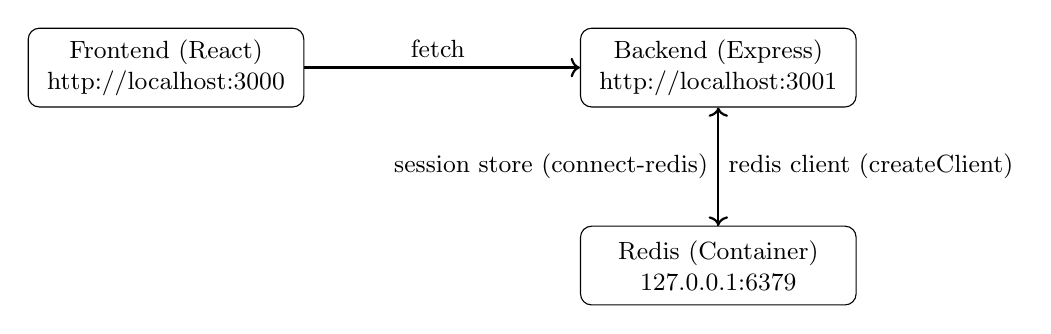
\begin{tikzpicture}[node distance=2cm, every node/.style={font=\small, align=center}]
  % nodes
  \node[draw, rectangle, rounded corners, minimum width=3.5cm, minimum height=1cm] (frontend) {Frontend (React)\\http://localhost:3000};
  \node[draw, rectangle, rounded corners, minimum width=3.5cm, minimum height=1cm, right=3.5cm of frontend] (backend) {Backend (Express)\\http://localhost:3001};
  \node[draw, rectangle, rounded corners, minimum width=3.5cm, minimum height=1cm, below=1.5cm of backend] (redis) {Redis (Container)\\127.0.0.1:6379};

  % arrows
  \draw[->, thick] (frontend.east) -- node[midway,above]{fetch } (backend.west);
  \draw[->, thick] (backend.south) -- node[midway,right]{redis client (createClient)} (redis.north);
  \draw[->, thick] (redis.north) -- node[midway,left]{session store (connect-redis)} (backend.south);
\end{tikzpicture}
\caption{Visão arquitetural simplificada}
\end{figure}

Observações específicas do projeto:
\begin{itemize}
\item O backend atual define a URL do redis em \texttt{server.js}\\
(exemplo: \texttt{redis://:your-strong-dev-pass@localhost:6379}). \\
Verifique a variável de ambiente \texttt{REDIS\_URL} em produção/testes.
\item As sessões são salvas com prefixo \texttt{sess:} por padrão (connect-redis).
Use comandos \texttt{SCAN} / \texttt{GET} no redis-cli para inspecionar.
\end{itemize}

\section{Infraestrutura}
Recomenda-se executar Redis via Docker Compose durante o desenvolvimento. 
Exemplo mínimo (adaptado do repositório):
\begin{verbatim}
# backend/docker-compose.yml (trecho)
version: '3.8'
services:
  redis:
    image: redis:7-alpine
    command:
      - redis-server
      - --bind
      - 0.0.0.0
      - --requirepass
      - "<your-dev-pass>"
      - --protected-mode
      - "yes"
    ports:
      - "127.0.0.1:6379:6379"
\end{verbatim}

Notas de segurança:
\begin{itemize}
\item Em desenvolvimento, publicar em \texttt{127.0.0.1} impede acesso direto da rede externa.
\item Em produção, evite publicar Redis ao público; prefira networking interno
(sem \texttt{ports:}) e autenticação forte.
\item Habilite ACLs/TLS em ambientes expostos.
\end{itemize}

\section{Metodologia de testes (protótipos)}
Objetivo: validar comportamento de sessões, latência e tolerância a falhas para o uso de Redis. A estratégia de testes segue três níveis:

\subsection{Testes unitários}
- Testes do código do backend (rotas, validação) com mocks do Redis. Use bibliotecas de testes do Node.js (Jest, Mocha).
- Mock do client Redis para verificar que a função de criação de sessão chama o método \texttt{req.session.save} corretamente.

\subsection{Testes de integração (local)}
- Subir Redis via docker-compose e executar testes que fazem requests reais ao backend.
- Verificar que, após login, existe uma chave \texttt{sess:*} no Redis. Comandos úteis:
\begin{verbatim}
# check keyspace
redis-cli -h 127.0.0.1 -p 6379 -a '<your-dev-pass>' INFO keyspace
# scan sessions
redis-cli -h 127.0.0.1 -p 6379 -a '<your-dev-pass>' \\
--scan --pattern 'sess:*'
\end{verbatim}

\subsection{Testes de carga / protótipo}
Cenários:
\begin{enumerate}[label=\arabic*)]
  \item Conexões concorrentes de login: medir latência e throughput quando N usuários tentam logar simultaneamente (por exemplo, N=100, 500, 1000).
  \item Persistência de sessão: conectar, confirmar sessão, reiniciar backend e confirmar que a sessão persiste em Redis (se esperado).
  \item Falha e recuperação do Redis: simular reinício do container Redis e verificar comportamento do backend (reconexão, erros de sessão).
\end{enumerate}

Ferramentas de teste:
\begin{itemize}
  \item Artillery (node) ou hey / wrk para carga HTTP.
  \item redis-benchmark para testes específicos de throughput em Redis.
\end{itemize}

Exemplo simples de comando Artillery (fluxo de login):
\begin{verbatim}
# Exemplo (instale artillery globalmente: npm i -g artillery)
# arquivo simple-login.yml
config:
  target: "http://localhost:3001"
  phases:
    - duration: 60
      arrivalRate: 20
scenarios:
  - flow:
      - post:
          url: "/api/auth/login"
          json:
            username: "user"
            password: "user123"
\end{verbatim}

\end{document}

